\chapter{Introduction}

\section{Overview}
\label{Intro: Overiew}
Dementia is a neurodegenerative condition that sees the deterioration of cognitive abilities, often leading to an increased dependence on care, leading to societal stereotyping and stigmatisation [5,50]. With dementia, the decline may change social functioning, judgement, problem-solving and may require care or other support to engage in social or complex activities. Given the vast complexities that a diagnosis presents, many of these can be seen as ethical concerns, making it a challenging space for both research and care practices. Traditional accounts of dementia often emphasize its biomedical origins (Leibing Annette 2006). As dementia progresses, it often adds conflict between the person and their surroundings as they can become unfamiliar, and this can also cause difficulties with coexisting with others; this can happen in what was previously a familiar space such as a family home, a local community, or work place (Au et al. 2009; Langdon et al. 2007). Challenges within previously familiar surroundings can cause issues for the person with dementia who may feel less able to express and explore their identity (John Killick Claire Craig 2012; Kontos 2005). As we live in a society that places a high value on cognitive ability, a diagnosis of dementia can put significant strain on meaningful interactions, relationships, and activities. 

Kitwood (1998) and others have followed person-centered approaches to dementia care and have called attention to how we communicate with people with dementia \citep{oyebode_mental_2005}, debated the need for ongoing consent processes \citep{dewing_participatory_2007}, questioned the contested use of lies and deception in care \citep{elvish_lying_2010} and promoted the need to attune to embodied, non-verbal communication \citep{group_patron_2019,twigg_dress_2013} as key considerations in ensuring the person with dementia is respected and engaged within their own care. These practices, largely initiated within nursing and social care, have implications for research and design which seeks to work with and for people living with dementia, avoiding practices that devalue or disregard the experience of the person living with dementia. \cite{john_killick_claire_craig_creativity_2012}, highlight the use of arts and creativity to provide alternatives to verbal communication that extends the importance of finding unique ways to offer people with dementia the opportunity to share their experiences. Through humour, dancing, acting, music, movement, and fashion, people living with dementia can evoke narratives and identities that can be particularly effective for those who may have their narratives' dissolve' as the condition develops. As the narrative of dementia continues to grow and change through the sharing of lived experiences, researchers must continue to explore ways to represent the voices of those who are continued to be underrepresented through creative ways to involve these individuals in the conversation and amplify their voices. \cite{swarbrick2015quest} argues research approaches should be more collaborative where people with dementia are recognised for their contribution. 


\subsection{Why must we broaden the conversation?}
\label{Design-conversation}
The shift in recognising the person with dementia's individuality emphasised the value in engaging and understanding the lived experiences and stories of people with dementia and their care partners. \cite{bartlett_personhood_2007} describes moving beyond solely individual values through a citizenship lens that recognises the potential power relationships that will likely stem from a diagnosis of dementia. The authors argue that a lens that considers not only the power dynamics but also the relationships to the person and the unique nature of the individual are all connections we must consider when reflecting on the dementia context. Moving towards a citizenship model has empowered and promoted people with dementia to share their experiences to make themselves more visible to impact policymaking, practice, and research \citep{weetch_involvement_2020}. The sharing of experiences has an impact in two ways. First, advocating and sharing experiences foster purpose and impact in understanding dementia on a more meaningful and inclusive level; and two, the stories promote awareness and improve public perception \citep{reynolds2017stigma}. 

Sharing lived experiences can also be seen in the recent proliferation of blogs, presentations, and personal books advocating for changes in media and public portrayals of dementia which might in turn counteract dominant misconceptions about, and stereotypes of, the condition [11, 13, 84].  While this creates an opportunity for public engagement, the extent to which the ‘public’ are engaging with these narratives is underexamined, begging the question: how can these experiences be better positioned for societal change-making? Moreover, such advocacy work, despite its benefits, is often associated with strain, through the \textit{``psycho-emotional consequences of taking action''} [2] where advocates present themselves in an opposing dominant public view. For instance, Christine Bryden, a pioneering dementia advocate, will often show images of her brain scans in presentations to prove she has dementia as several advocates have been accused by medical practitioners of not \textit{``look[ing] or sound[ing] like [they] have dementia''} [83]. In these instances, exploring ways to balance between empathy and maintaining an individual’s privacy and dignity is required.

To an extent, improving public perception and citizenship approach resonates with policy and practice. In 2020, the UK set out the Prime Minister's challenge to make England the best place to live with dementia, and be the leading place in the world for dementia research \citep{budgett2021designing}. This challenge is set out to tackle: dementia-friendly health and care settings; educate people earlier about the risks of developing dementia; and provide more opportunities for people with dementia to partake in research and present talks about their experiences. \cite{keady2017social} argues that these aims by the UK present dementia as \textit{``everyone's business and responsibility, from architects to town planners, public transport providers to shop owners, next-door neighbours on the street where the person with dementia lives - the list is seemingly endless''}. As such, given that dementia is part of a complex ecology of care, which considers the person with dementia, friends, family, healthcare systems, researchers, designers and everyday interactions, it is particularly timely to unpack what it means to design methodologies that take into account the multivariate stakeholders and infrastructures that surround and often hold up our work. For the thesis, I focus on broadening the conversation regarding designing technology with people with dementia - that considers the type of methods and tools to promote conversation between people with dementia, family members, designers, developers, and researchers.

\section{Research context}
\label{Intro: ResearchContext}
Early HCI and dementia work has evolved our understanding of dementia by focusing on how we involve people with dementia in technology design processes [6,58,88,93,95,96]. For instance, Wallace et al. use a tailored approach that centred on the importance of personhood by paying attention to a person’s individual and unique experiences of dementia to design bespoke digital artifacts for the participants [96]. Similarly, Lindsay et al. describes the need for more interpretative data approaches for those at later stages of dementia, which in turn, may require longer-term projects and relationships to form throughout a study [58]. This early work stresses the required need to adapt co-design and participatory approaches to accommodate the different communication needs of people with dementia, ensuring they are respected rather than infantilised [68,70,80]. 

More recent work has seen a critical turn to understanding personhood even in the presence of later stages of dementia, where non-verbal and ambiguous interactions may be more present [41]. Treadaway and Kenning emphasise that recognition and appreciation are crucial even when leaning on tacit, creative activities to support non-verbal interactions [92]. This critical turn is further supported in work by Morrissey et al, taking an experience-centred approach that shifts the way we see people with dementia-related cognitive deficits as contributing to design choices [67]. While prior work may focus on alleviating a person's cognitive deficit, the critical perspective widens our approach to inclusivity, by celebrating what a person has to offer through more creative and engaging approaches, where those living with a broad spectrum of dementia-related changes can also participate [54].
To help foster empathy with, and understanding of, a person with dementia's experience, there has been a push from dementia activists towards using online interactions and bespoke forums and Twitter to raise awareness and further challenge the stigma surrounding dementia [89]. Dai and Moffatt’s recent work on social sharing through community-based programs describes how future platforms involving people with dementia need to allow flexibility for "dynamic roles" where individuals can flip between "storytellings, listeners, contributors" as the "activities [on the platform] evolve" (pg.10) [25]. Likewise, Johnson et al. argue that these roles may need support from "various stakeholders in participating without burdening" (pg.127) people with dementia [45,46]. The further involvement of gatekeeping stakeholders may provide useful moderation and provide safety and familiarity on online spaces that can feature bad actors who target the vulnerability of people with dementia. 

This move to online-mediated change-making mirrors a trend in work on participatory platforms and digital civics that has begun examining and developing tools to promote change and support marginalised voices [21]. For instance, Puussaar et al. developed a visual map-based querying tool to provide the public to interpret and understand open-source datasets that are typically incomprehensible by non-professionals [76]. Asad’s work on similar civic platforms describes that there is an "obligation [for] designers and researchers to ensure our work aligns with existing efforts in our respective research communities" (pg. 6314) [3]. In Foley et al.'s work on student engagement within dementia care, the authors describe that over time, students started to take "responsibility for the development of the relationships" while the person with dementia was "viewed as experts, with knowledge and stories to share beyond their role as a patient in care" (pg.9) [29]. However, to support collaboration and engagement between those who are being designed for, and those who are doing the designing, we need further consideration into the articulated needs and desires of such platform users - particularly those within socially complex contexts. 

In response, the thesis explores \textit{``How might participation be configured for people with dementia to shape the design process of technology?''} From the literature review, I describe that research involving people with dementia requires adaptability to ensure inclusive and meaningful engagement. In turn, this raises the question of what approaches should consider for designers and developers that allow them to design with people with dementia collaboratively. Building on the literature, the thesis describes four studies involving diverse stakeholder's perspectives who are commonly part of the design process when designing for and with people with dementia. Through this, the thesis iteratively explores the competing interests and expectations for involving the stakeholders to question how collaboration might fit into the different practices. Within each study, the findings and discussion sections contribute new knowledge concerning how participation is adapted and shaped to develop inclusive design spaces that support mutuality in the co-creation of new technologies and systems.


\section{Research aim and questions}
\label{Intro:RQ}
The research described in this thesis explores the following research aim:
\begin{quote}
    \textit{``How might participation be configured for people with dementia to shape the design process of technology?''}
\end{quote}
This research aim is split into three research questions, to provide insights into the experiences and perspectives of stakeholders commonly implicated in design processes in designing with and for people with dementia, intending to broaden the conversation surrounding technology design with and for people with dementia. The following section introduces each research question followed by a description.

\subsection{Research question one}
\label{RQ1}
\begin{quote}
\textit{``How can we use participatory design approaches to provide meaningful and engaging experiences for people with dementia?''}
\end{quote}
In exploring this question, the methodologies used in this thesis explore the ways to move toward more inclusive design approaches that require flexible configuration to support the different needs of participants. Further, this exploration draws attention to how we talk about dementia, to what extent people with dementia want to contribute to technology design, and ways to ensure the person with dementia is respected and engaged in research.

\subsection{Research question two}
\label{RQ2}
\begin{quote}
\textit{``What are the ethical implications for people with dementia to participate in HCI research?''}
\end{quote}
Given that people with dementia may experience changes to their ability to problem solve, increasing need for care, and make judgements, many of the social and cognitive consequences of living with dementia can be seen as ethical challenges, making it a complex space for research. With this in mind, the thesis examines ethical practices used in dementia-HCI research to present insights into the careful ethical considerations required when working with people with dementia and their families. 

\subsection{Research question three}
\label{RQ3}
\begin{quote}
\textit{``What are the competing interests and expectations to support meaningful dialogue in dementia design research when involving multiple stakeholders - such as people with dementia, developers, designers and researchers?''}
\end{quote}
For the final research question, the thesis investigates the importance of designing for multiple interests and workflows to ensure that stakeholders who are part of the design process to support collaboration and engagement between the diverse stakeholders. 

\section{Thesis structure}
\label{Intro: Thesis structure}
In this section, I describe the structure of the thesis:

\subsection{Chapter two - Background Literature}
\label{Intro:ChapterTwo}
This chapter aims to describe prior work discussing how people with dementia have been represented and involved in technology design and development. Initially, this chapter reviews the involvement of people with dementia in dementia-HCI work that draws attention to a strong relational basis for design practice. Following the review of dementia-HCI work, I highlight three areas that require investigation. From here, I draw from outside the HCI literature that examines the type of ethical dilemmas; public perception of dementia, and involving later stages of dementia in the co-creation process. Finally, to conclude this chapter, I describe four areas of interest to this thesis that might broaden our understanding of how to design and develop technology for and with people with dementia.

\subsection{Chapter three - Methodology}
\label{Intro:ChapterThree}
In the methodology chapter, I explain and justify the research approach taken in the thesis that shapes the data chapters. First, I introduce the epistemological approach adopted in this thesis. Following, I describe how I adapt co-design and participatory design to fit the needs of people with dementia. I then unpack participatory methods in dementia and HCI that emphasise the need to adopt approaches to fit the needs of people with dementia. I discuss the ethical complexities of the thesis; the data collection of the four data chapters; overview of recruitment and location; and the qualitative data analysis method, thematic analysis and reflexive practice. Moreover, I detail the analytical and reliability approaches I undertake in this thesis to provide work that is more mindful of the assumptions and methodological choices made within this thesis.

\subsection{Chapter four - Sharing a Virtual World with People with Dementia: A Reflective Account}
\label{Intro:ChapterFour}
The chapter is a reflective account highlighting several themes and reasons for the subsequent chapters. This chapter reflects on two studies working with people with dementia and their families to design virtual reality experiences. Both studies worked closely with a dementia café in Newcastle called Silverline Memories, which provide activities and organise celebrations for members' birthdays and other special occasions. By working closely with families with dementia, the account examines how I adapted participatory approaches to involve people with dementia in more sensitive and meaningful ways. Further, by working with family members as well as the person with dementia, I recognise that many of the challenges in designing technology with people with dementia should consider the needs and interests of the ecology of care. In that respect, this chapter takes a reflective approach to provide a clear account of my background, history, the perspective on dementia, and design approaches that ultimately impact the participants, the setting and the overarching work. As such, this chapter provides insights into designing VR environments for families with dementia and a personal narrative, that recognises the concerns, dilemmas, and the impact of working within sensitive research spaces.

\subsection{Chapter five - DemVR: Exploring Shifting Sensitivities in a Hackathon for Dementia}
\label{Intro:ChapterFive}
Following the two studies focusing on the inclusive design of virtual reality experiences for families living with dementia, I was curious about how designing bespoke and sensitive VR experiences might function in larger-scale community events. As I described in chapter four, learning to design within such a complex topic required extensive time working with people with dementia. However, developers and designers who work on bringing dementia technology to the market, will unlikely have the chance to work with people with dementia to the extent I could. As such, this chapter explores the design of a hackathon, DemVR, both to generate a set of bespoke VR environments for those with dementia and consider how developers/designers and people with dementia may collaborate.

The event consists of two stages: a six-week engagement phase to support participants in proposing and refining initial ideas online; and a two-day hackathon inviting designers and domain experts to develop their ideas further. While the event gained reasonable interest from designers, developers, and students throughout both phases, the representation of people with dementia and their care partners was limited. The chapter examines the structure of the event and the role this played in the struggle to involve people with dementia and their care partners. The data analysis presents insights into participants’ motivations, design approaches to accommodate the absent user, and the design ideas that the teams developed to address the social context of the user. Against a background of the extant literature on reification in design, collaborative design events, and dementia, the discussion provides a series of commitments for HCI and dementia research. The commitments offer insights into how we might mitigate stereotypes in constructing the end-user; ways to improve recruitment for involving marginalised populations in events; and steps to promote more inclusive, community-driven events. 

\subsection{Chapter six - Learning from Ethics in Dementia Research}
\label{Intro:ChapterSix}
From work in chapter four and five, I highlighted several topics regarding the ethical challenges when working in dementia and HCI. Similarly, these challenges resonated with recent work by HCI researchers. For instance, academics in the HCI field often reflect on the ethical challenges they face throughout their research process, with conversations predominantly occurring in venues such as Town Halls and conference workshops at ACM venues.

This chapter provides an analysis of the accounts of 22 researchers working in dementia design research. The analysis of interviews raises numerous ethical complexities such as consent, participation recognition, self-care, and researcher relationships. Further, the findings examines the potential challenges researchers face with Ethical Review Boards (ERB), who, while prioritising the protection of human subjects, can inadvertently bar the full inclusion of people living with dementia in socially-oriented research. I proceed from the findings to emphasise a set of directions for researchers and ethical review boards to improve their practices by moving towards more participant-led research, re-framing impact and aiming for research clarity.

\subsection{Chapter seven - Co-creating a Digital Toolkit to Support Design for Dementia}
\label{Intro:ChapterSeven}
From the data analysed in the previous chapters, it was apparent that a) representing people with dementia can be difficult in public events and causes multiple knock-on effects on design outputs; and b) future research work in dementia should aim to be participant-led and shift towards creating tools or processes to promote conversations between people with dementia and stakeholders commonly implicated in design processes.

In response, this chapter presents the design of the Dialogical Dementia Design (D3) toolkit, a set of resources to support co-designing with people with dementia. The study invited designers and developers and people with dementia to participate in interactive workshops and interviews that explored resources needed by developers and designers to design with people with dementia and investigate how people with dementia envision their potential participation with toolkits. Through iterative engagement with participant data, I surfaced a set of design priorities that helped shape a prototype of the toolkit. This toolkit comprised several components that offered opportunities to learn and engage in sensitive ways with people with dementia. Analysis of participant reactions to the designed prototype raises questions around the challenges of co-creation through safety and privacy, the sharing of the ‘designer’ role between the different stakeholders, and finally, the type of incentives required for participation and engagement in curating a toolkit. Against a background of extant literature on dementia and collaboration, the discussion provides a series of directions for HCI and dementia research, highlighting how we might balance participants' privacy, safety, and due recognition; priorities in growing a community-owned toolkit; and the accountability and responsibility that designers and developers carry in adapting their working practices for designing within sensitive areas.
\subsection{Chapter eight - Discussion and Future Work}
\label{Intro:ChapterEight}
In the final chapter, I synthesise the findings from the data chapters by returning to answer the research questions I set out at the start of this thesis. The discussion aims to answer how researchers adapt participation approaches to provide more engaging experiences for people with dementia; how, as researchers, can we mitigate some of the ethical implications for when people with dementia participate in HCI research; and how can we balance and design for the competing interests and expectations of diverse stakeholders to ensure the support of meaningful dialogue between people with dementia, designers and developers. The chapter concludes with suggestions for future work that I organise into a design approach consisting of three core components that reimagine the role of participation between people with dementia and stakeholders. By considering the three components, the approach aims to move towards more inclusive design spaces that support mutuality in the co-creation of new technologies and systems.

\newpage
\subsection{Thesis map}
For chapters four to seven, I present a map of which represents the different research questions each data chapter tackles (see figure \ref{fig:RQ_and_Chapters}).

\label{Intro:Thesis Map}
\begin{figure}[htp]
\centering
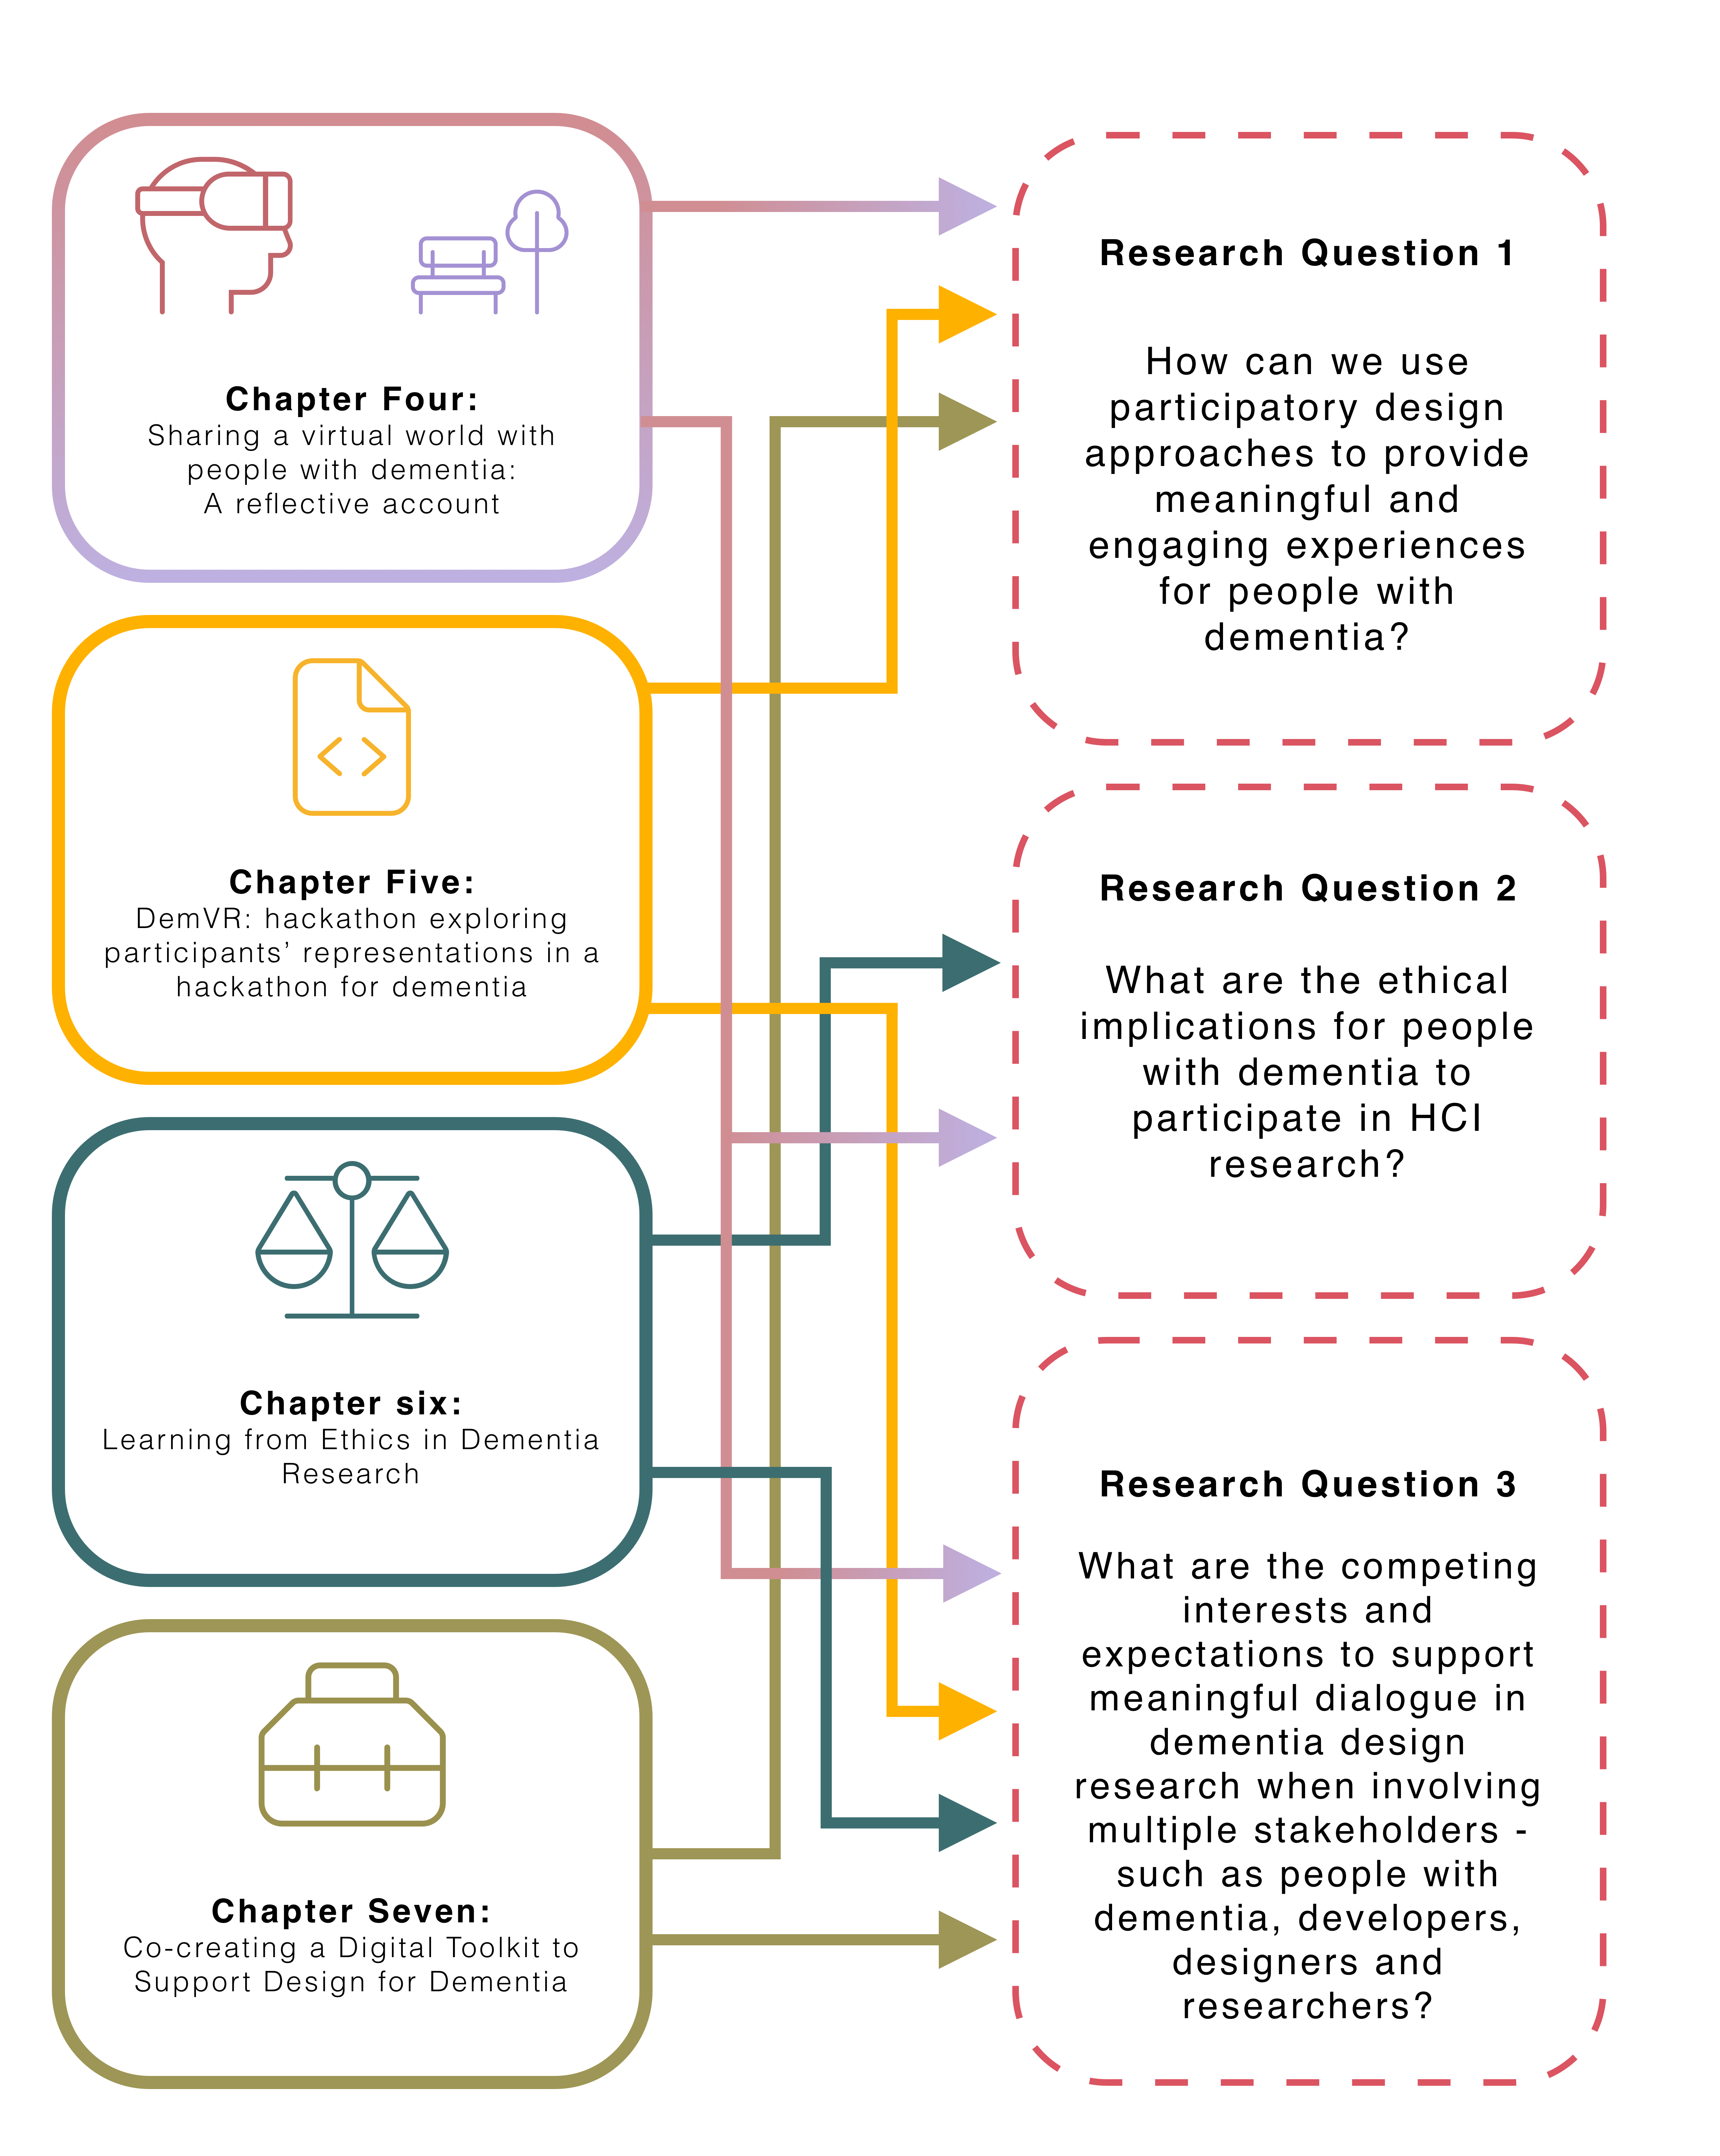
\includegraphics[width=.8\linewidth]{Images/Thesis_Narrative/RQ_and_Chapters.png}
\caption{Thesis Map showing the relationships between data chapters to research questions}
\label{fig:RQ_and_Chapters}
\end{figure}


\section{Contributions}
\label{Intro:Contribution}
In addition to the thesis resulting in a number of publications (see x), the thesis offers three contributions to knowledge in dementia and HCI:

\begin{itemize}
    \item \textbf{Empirical contribution}: This thesis uses data collected through walking interviews, workshops, hackathon event, and semi-structured interviews to provide qualitative insights into the experiences and perspectives of a diverse set of stakeholders implicated in design processes in designing with and for people with dementia. Through the findings gained across the data chapters, this thesis advances an understanding of the ethical and practical requirements to promote conversation and inclusion of stakeholders surrounding technology design with and for people with dementia. This thesis offers practical examples and directions for future HCI work in design spaces that support mutuality in the co-creation of new technologies and systems
    
    \item \textbf{Artefact contribution}: Within the thesis, two chapters consist of novel systems and prototypes to facilitate new insights and consider ways for people with dementia to engage with technology and contribute to the design process. In chapter four, I use the design of virtual reality environment prototypes to explore the ways people with dementia might use this novel technology. Through this work, the prototypes provide an understanding of the desire for shared experiences and how the sensitive capture and curation of digital media can help to keep the experience alive for people with dementia who might seek to experience such media `in the moment', in shared social contexts. 
    
    In chapter seven, I collaborated with designers, developers and people with dementia to develop a lo-fi prototype toolkit to support designers and developers in co-design with people with dementia. The main contribution of this work, provides a series of directions for HCI and dementia research highlighting how we might balance participants' privacy, safety, and recognition; priorities to contribute and grow a community-owned toolkit; and the accountability and responsibility that designers and developers carry when designing in such sensitive and ever-changing situations.
    
    \item \textbf{Methodological contribution}:  The thesis contributes to a methodological understanding of how supporting participant-led methods provides more engaging and expressive design approaches. In chapter four, by inviting families to a set of walking interviews (also known as days out), the families could communicate in ways beyond verbal interaction by taking the lead of the walk and using non-verbal expression to contribute to the research. Additionally, this contribution stresses the challenges I faced in running a platform for online engagement for people with dementia and care partners in chapter five. By reflecting on how the approach led to a lack of involvement by people with dementia, this chapter provides ways to improve recruitment for involving marginalised populations in hackathons.
\end{itemize}
